
\subsubsection{G.711}

El códec básico y más antiguo en telefonía es el estandarizado en la recomendación G.711 de la ITU-T, está enfocado en reproducir la “forma de onda” de la señal y su cuantificación, de tipo “no lineal” puede hacerse de acuerdo a dos leyes, “ley A” o “ley u” \cite{g711}. 

Como G.711 es un códec de banda angosta, su frecuencia de muestreo es de 8kHz, es decir, se toma una muestra cada 125 microsegundos. Si bien esta frecuencia es adecuada para reproducir la voz humana, con cierto grado de perdida, no es adecuada para audio de alta calidad con frecuencias máximas de 20kHz.

Se ha demostrado que el oído humano es más sensible a ruidos en señales de baja amplitud que a los mismos ruidos en señales de mayor amplitud. Por lo tanto, al tener una cuantificación de tipo “no lineal” se acepta tener distorsiones grandes en las partes de mayor amplitud de la señal mientras que en las partes de baja amplitud de la señal las distorsiones sean más pequeñas. 

Tanto la cuantificación como la codificación de las señales, con éste códec, dependen directamente de la ley implementada. Estas “leyes de compresión” estandarizan en 256 niveles no lineales la cuantificación y codificación de la voz en telefonía basadas en fórmulas matemáticas bien definidas, sin embargo la implementación real utiliza 13 segmentos de recta que se aproximan a la formula teórica de la “Ley A” y 15 segmentos aproximados a la formula teórica de la “Ley u“. Para información más detallada de cada ley se sugiere revisar la recomendación G.711 \cite{g711}.

\subsubsection{G.711.1}

El códec G.711.1 es una extensión a banda amplia del códec original G.711. En su modo “banda amplia” codifica señales de hasta 7kHz y está optimizado para VoIP. Una característica interesante de este códec es su compatibilidad hacia atrás. Por lo que toma muestras a 16kHz en su modo amplio y a 8kHz en su modo de compatibilidad. Las tramas son de 5ms por lo que la perdida de paquetes no afecta en gran medida a la reconstrucción de la señal. En la siguiente [FIGURA \ref{fig:g7111}]\footnote{Extraído de www.adaptivedigital.com/products/vocoders/g.711.1.pdf} se puede apreciar los modos de operación de este códec.

	\begin{figure}[h]
		%nombre de la imagen, sin extencion. "width=\textwidth" ancho igual al texto
		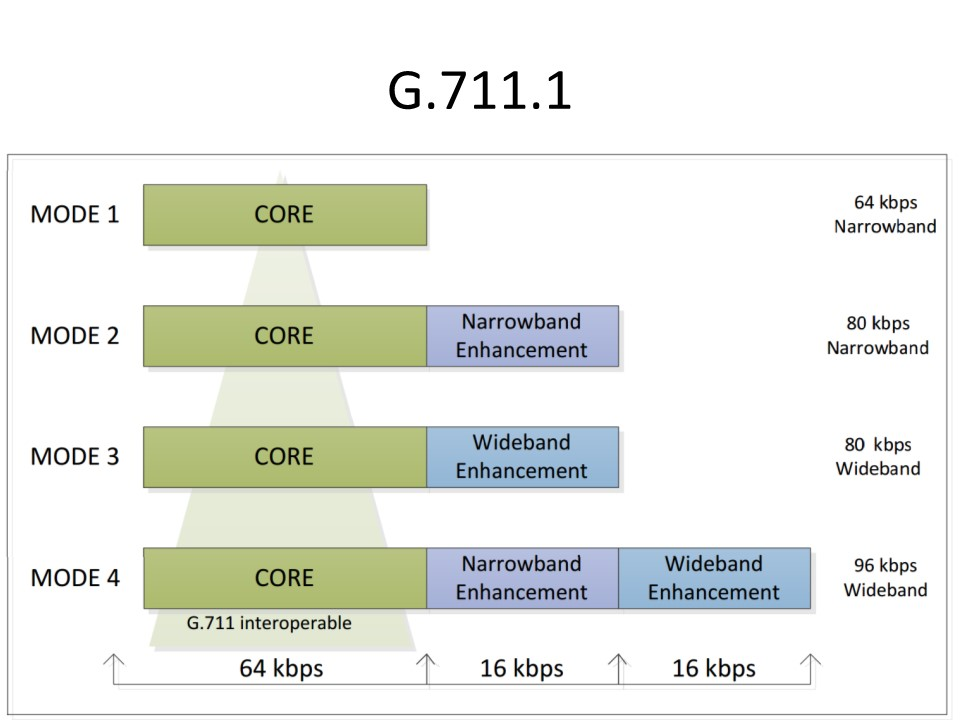
\includegraphics[width=\textwidth]{g7111}
		
		%titulo de la imagen, salen debajo de la imagen y en el indice de imagenes.
		\caption{Modos de operación del G.711.1}
		
		%centrado, por si las moscas
		\centering
		
		%para referencias
		\label{fig:g7111}
	\end{figure}

\subsubsection{G.722}
El códec G.722 separa la señal de audio en dos bandas y las codifica por separado usando la técnica ADPCM (Adaptative Differential Pulse Code Modulation). Puede operar  a veocidades de 64, 56 y 48 kbits/s. En los últimos dos casos es posible enviar un canal auxiliar de información de 8 o 16 kbit/s respectivamente, completando así una velocidad constante de 64kbit/s.

\subsubsection{G.723.1}
El códec G.723.1 codifica las señales de voz a 6,4 o 5,3 kbit/s usando ventanas de 30ms. Para la velocidad de 6,4 kbit/s utiliza el algoritmo MP-MLQ (Multi-Pulse Maximun Likelihood Quantization), generando 24 bytes de datos por cada ventana de 30ms. Para la velocidad de 5,3 kbit/s se utiliza ACELP, generando 20 bytes por cada ventana de 30ms (Algebraic Code Excited Linear Prediction).

El anexo A de la recomendación G.723.1 ayuda a reducir el ancho de banda utilizado al no transmitir muestras durante los periodos de silencio.

\subsubsection{G.729}
El códec G.729 codifica las señales a 8 kbit/s utilizando CS-ACELP (Conjugate-Structure Algebraic-Code-Exited Liner Prediction). Utiliza ventanas de 10ms generando 10 bytes de datos por ventana.

El Anexo A del códec define una variante que reduce su complejidad y es compatible hacia atrás con el códec original.

El Anexo B de la recomendación G.729 provee detección de actividad de voz y silencios, ayudando a disminuir el ancho de banda utilizado al no enviar muestras durante los periodos de silencio.

\subsubsection{G.729.1}
El códec G.729.1 amplia el espectro de frecuencias del códec G.729. Fue diseñado para facilitar la interoperabilidad entre las redes de banda angosta (300 a 3400 Hz) y las redes de banda ancha (50 a 7000 Hz). 
La señal codificada tiene una tasa de bits de 8 a 12 kbit/s para señales de banda angosta y de 14 a 32 kbit/s para señales de banda ancha. Las tramas de salida consisten en 12 capas, como se muestra en la [FIGURA \ref{fig:g7291}]. 

\begin{figure}[h]
	%nombre de la imagen, sin extencion. "width=\textwidth" ancho igual al texto
	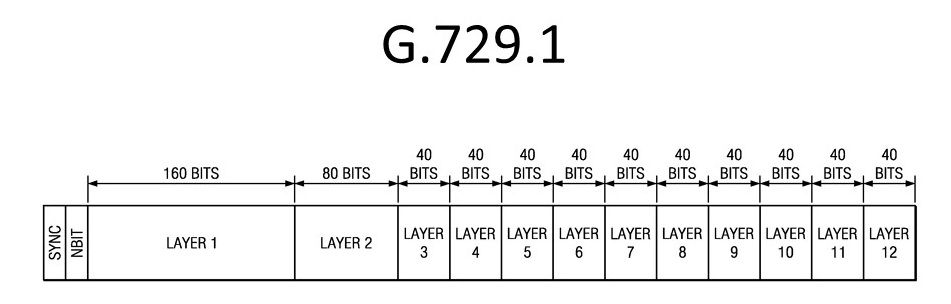
\includegraphics[width=\textwidth]{g7291}
	
	%titulo de la imagen, salen debajo de la imagen y en el indice de imagenes.
	\caption{Capas del códec G.729.1}
	
	%centrado, por si las moscas
	\centering
	
	%para referencias
	\label{fig:g7291}
\end{figure}

La capa 1 corresponde a 8 kbit/s y utiliza la codificación CELP, siendo compatible con G.729. La capa ocupa 4kbit/s y corresponde a mejoras en las frecuencias de la banda angosta. Las siguientes capas ocupan 2kbit/s cada una y corresponden a mejoras en las frecuencias de banda ancha.

Las tramas son de 20ms y puede ser truncada a la salida del codificador, en el decodificador, o cualquier otro punto de la red, si fuera necesario reducir el ancho de banda.

\subsubsection{RTAudio}
El códec RTAudio fue desarrollado por Microsoft y ha sido usado comercial y cooperativamente. Utiliza 8,8 kbit/s de ancho de banda y técnicas LPC (Linear Prediction Coefficients). RTAudio utiliza técnicas VBR (Variable Bit Rate), lo que significa que no todas las ventanas o muestras se codifican con la misma cantidad de bytes.

\subsubsection{SILK}
El códec SILK fue utilizado por SKYPE. Utiliza un ancho de banda variable, entre  6 y 40 kbit/s. Éste códec puede trabajar en banda angosta y banda ancha, con tramas de 20 ms y un retardo de 25 ms.
 
SILK fue reemplazado por el códec OPUS, el cual fue aceptado con el RFC 6716--REFERENCIA NECESARIA.  

